\graphicspath{{images/}}

\section{Determinante}

    \begin{definition}{Determinante}\\
        Die Determinante gibt an, ob eine Matrix invertierbar ist.
        \begin{equation*}
            \det(A)
            \left\{
                \begin{array}{lll}
                    \neq 0   &\Rightarrow    & A^{-1} \text{ existiert. }\\
                    = 0     &\Rightarrow    & A^{-1} \text{ existiert nicht. }
                \end{array}
            \right.
        \end{equation*}
    \end{definition}

    

    \begin{definition}{Geometrische Interpretation} der Determinante:\\
        \begin{minipage}{0.6\linewidth}
        \begin{itemize}
            \item Fläche im $\mathbb{R}^2$
            \item Volumen im $\mathbb{R}^3$
        \end{itemize}
        welche durch eine Matrix A aufgespannt wird.
        $$A = |\vec{a} \times \vec{b}| = |\det(A)|$$
        \end{minipage}
        \begin{minipage}{0.35\linewidth}
            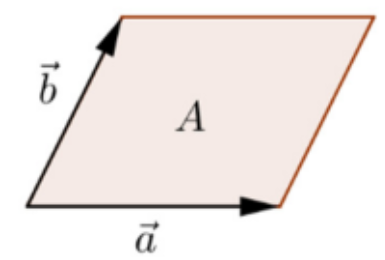
\includegraphics[width=0.9\linewidth]{determinante.png}
        \end{minipage}
    \end{definition}

    \begin{theorem}{Geometrische bedeutung der Determinante}


        \begin{wrapfigure}[16]{hr!}{0.35\textwidth}
            \vspace{-10pt}
            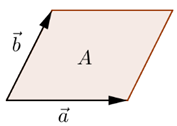
\includegraphics[width=0.9\linewidth]{det-vis-2d.png}
            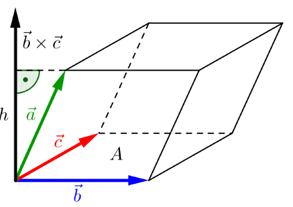
\includegraphics[width=0.9\linewidth]{det-vis-3d.png}
        \end{wrapfigure}
        Die Spalten einer $2\times 2$-Matrix $A$ spannen ein Parallelogram auf.
        Die Determinante der Matrix $A$ ist dabei gerade der \textbf{Flächeninhalt} des aufgespannte Parallelogram.
        \vspace{1.25em}

        Werden Spalten einer $3\times 3$-Matrix $B$ als raum Vektoren betrachtet, 
        spannen diese einen Spat auf.
        Die Determinante der Matrix $A$ ist dabei gerade das $Volumen$ des aufgespannten Spat.
        \vspace{1em}
    \end{theorem}
    
    \begin{theorem}{Determinantenregeln}\\
        \begin{minipage}{0.5\linewidth}
            \begin{itemize}
                \item $\det(A) = \det(A^T)$
                \item $\det(A \cdot B) = \det(A) \cdot \det(B)$
                \item $\det(A^{-1}) = \frac{1}{\det(A)}$
            \end{itemize}
        \end{minipage}
        \begin{minipage}{0.5\linewidth}
            \begin{itemize}
                \item $\det(\lambda \cdot A) = \lambda^n \cdot \det(A)$
                \item $\det(A) = 0 \Leftrightarrow A$ ist singulär
            \end{itemize}
        \end{minipage}
    \end{theorem}

    \begin{theorem}{Eigenschaften von Determinanten}
        Gegeben zweier \textit{quadratischer Matrizen} $A$, $B$ 
        sowie einer \textit{quadratischen Dreiecksmatrix} $D$.
        \begin{align*}
            &\det(E)        &&=1                     \\
            &\det(D)        &&=\prod_{i=1}^n d_{ii}  \\
            &\det(A\cdot B) &&=\det(A)\cdot\det(B)   \\
            &\det(A^T)      &&=\det(A)               \\
            &\det(A^{-1})   &&=\frac{1}{\det(A)}     \\
            &\det(m\cdot A) &&=m^n\cdot\det(A)\, \text{ mit } m\in \R
        \end{align*}
    \end{theorem}

    \begin{formula}{Determinante einer $1\times 1$-Matrix} $\det(A)=A_{11}$
    \end{formula}
    
    \begin{formula}{Determinante einer $2 \times 2$-Matrix}
        $A = \begin{pmatrix} a & b \\ c & d \end{pmatrix}$
        \begin{itemize}
            \item $\det(A) = |A| = a \cdot d - b \cdot c$
        \end{itemize}
    \end{formula}
    
    \begin{formula}{Determinante einer $3 \times 3$-Matrix}
        $A = \begin{pmatrix} a & b & c \\ d & e & f \\ g & h & i \end{pmatrix}$\\
        \begin{minipage}{0.4\linewidth}
            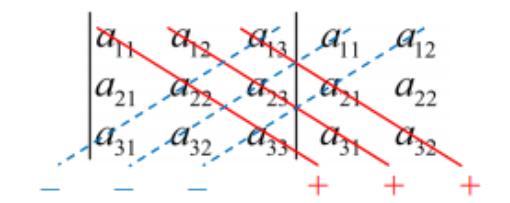
\includegraphics[width=0.8\linewidth]{determinante_3x3.png}
        \end{minipage}
        \begin{minipage}{0.5\linewidth}
            $|A| = a \cdot e \cdot i + b \cdot f \cdot g + c \cdot d \cdot h - c \cdot e \cdot g - b \cdot d \cdot i - a \cdot f \cdot h$
        \end{minipage}
    \end{formula}
    
    \begin{concept}{Determinante einer $ n \times n$-Matrix} $A$
        $$\det(A) = |A| = \sum_{j=1}^{n} (-1)^{i+j} \cdot a_{ij} \cdot |A_{ij}|$$
        \begin{itemize}
            \item Tipp: Entwickeln nach Spalte oder Zeile mit den meisten Nullen
            \item $|A_{ij}|$ ist die Determinante der $(n-1) \times (n-1)$-Matrix, die entsteht
        \end{itemize}
        evtl. bsp hier
    \end{concept}

    \begin{formula}{Determinante einer $n\times n$-Matrix nach Laplace}\\
        Gegeben einer $n\times n$-Matrix $A$, 
        wird zum berechnen der Determinante eine feste Zeile $i$ oder Spalte $j$ gewählt,
        nachder die Determinante entwickelt wird.

        \textbf{Entwicklung nach Zeile}
        \[\det(A)=\sum_{j=1}^n{(-1)}^{i+j}\cdot A_{ij}\cdot\det(A_{ij})\]
        \textbf{Entwicklung nach Spalte}
        \[\det(A)=\sum_{i=1}^n{(-1)}^{i+j}\cdot A_{ij}\cdot\det(A_{ij})\]

        Bezeichnungen:
        \begin{itemize}
            \item $a_{ij}$ ist das Element der Matrix $A$ in der $i$-ten Zeile und $j$-ten Splate
            \item $A_{ij}$ ist die Matrix, die durch das Weglassen der $i$-ten Zeile und $j$-ten Spalte entsteht. 
        \end{itemize}

        \begin{highlight}{!}
            Um den Rechenaufwand zu minimieren, entwickelt man nach derjenigen Zeile oder Spalte, 
            in der die meisten Nullen stehen. 
        \end{highlight}
    \end{formula}




\begin{theorem}{Lineare Abhängigkeit}
    Die folgenden Aussagen sind äquivalent:
    \begin{itemize}
    \item $\operatorname{det}(A) \neq 0$
    \item Spalten von $A$ sind linear unabhängig
    \item Zeilen von $A$ sind linear unabhängig
    \item $r g(A)=n$
    \item $A$ ist invertierbar
    \item Das LGS $A \cdot \vec{x}=\vec{c}$ hat eine eindeutige Lösung
    \end{itemize}
\end{theorem}

